\section{Density, Mass, and Center of Mass} \label{S:6.4.Mass}

\begin{goals}
\item How are mass, density, and volume related?  
\item How is the mass of an object with varying density computed?
\item What is the center of mass of an object, and how are definite integrals used to compute it?
\end{goals}

%-----------------------------------
% SUBSECTION INTRODUCTION
%-----------------------------------
\subsection*{Introduction}

We have seen in several different circumstances how studying the units on the integrand and variable of integration enables us to better understand the meaning of a definite integral.  For instance, if $v(t)$ is the velocity of an object moving along an axis, measured in feet per second, while $t$ measures time in seconds, then both the definite integral and its Riemann sum approximation,
$$\int_a^b v(t) \, dt \approx \sum_{i=1}^n v(t_i) \triangle t,$$
have their overall units given by the product of the units of $v(t)$ and $t$: 
\begin{center}(feet/sec)$\cdot$(sec) = feet.
\end{center}
Thus, $\int_a^b v(t) \, dt$ measures the total change in position (in feet) of the moving object.  

This type of unit analysis will be particularly helpful to us in what follows.  To begin, in the following preview activity we consider two different definite integrals where the integrand is a function that measures how a particular quantity is distributed over a region and think about how the units on the integrand and the variable of integration indicate the meaning of the integral.

\begin{pa} \label{PA:6.4}  In each of the following scenarios, we consider the distribution of a quantity along an axis.

\ba
\item Suppose that the function $c(x) = 200 + 100 e^{-0.1x}$ models the density of traffic on a straight road, measured in cars per mile, where $x$ is number of miles east of a major interchange, and consider the definite integral $\int_0^2 (200 + 100 e^{-0.1x}) \, dx$.
\begin{itemize}
\item[i.] What are the units on the product $c(x) \cdot \triangle x$?
\item[ii.] What are the units on the definite integral and its Riemann sum approximation given by
$$\int_0^2 c(x) \, dx \approx \sum_{i=1}^n c(x_i) \triangle x?$$
\item[iii.] Evaluate the definite integral $\int_0^2 c(x) \, dx = \int_0^2 (200 + 100 e^{-0.1x}) \, dx$ and write one sentence to explain the meaning of the value you find.
\end{itemize}
\item On a 6 foot long shelf filled with books, the function $B$ models the distribution of the weight of the books, measured in pounds per inch, where $x$ is the number of inches from the left end of the bookshelf.  Let $B(x)$ be given by the rule $B(x) = 0.5 + \frac{1}{(x+1)^2}$.
\begin{itemize}
\item[i.] What are the units on the product $B(x) \cdot \triangle x$?
\item[ii.] What are the units on the definite integral and its Riemann sum approximation given by
$$\int_{12}^{36} B(x) \, dx \approx \sum_{i=1}^n B(x_i) \triangle x?$$
\item[iii.] Evaluate the definite integral $\int_{0}^{72} B(x) \, dx = \int_0^{72} (0.5 + \frac{1}{(x+1)^2}) \, dx$ and write one sentence to explain the meaning of the value you find.
\end{itemize}
\ea
\end{pa} 
\afterpa % PREVIEW

%---------------------------
% SUBSECTION DENSITY
%---------------------------
\subsection*{Density} \index{density}

The \emph{mass} \index{mass} of a quantity, typically measured in metric units such as grams or kilograms, is a measure of the amount of a quantity.  In a corresponding way, the \emph{density} of an object measures the distribution of mass per unit volume.  For instance, if a brick has mass $3$ kg and volume $0.002$ m$^3$, then the density of the brick is 
$$\frac{3 \mbox{kg}}{0.002 \mbox{m}^3} = 1500 \frac{\mbox{kg}}{\mbox{m}^3}.$$
As another example, the mass density of water is $1000$ kg/m$^3$.  Each of these relationships demonstrate the following general principle.  

\concept{Density, Mass, \& Volume}{ % CONCEPT
For an object of constant density $d$, with mass $m$ and volume $V$, 
$$d = \frac{m}{V}, \ \mbox{or} \ m = d \cdot V.$$
} % end concept

But what happens when the density is not constant?

If we consider the formula $m = d \cdot V$, it is reminiscent of two other equations that we have used frequently in recent work:  for a body moving in a fixed direction, distance = rate $\cdot$ time, and, for a rectangle, its area is given by $A = l \cdot w$.  These formulas hold when the principal quantities involved, such as the rate the body moves and the height of the rectangle, are \emph{constant}.  When these quantities are not constant, we have turned to the definite integral for assistance.  The main idea in each situation is that by working with small slices of the quantity that is varying, we can use a definite integral to add up the values of small pieces on which the quantity of interest (such as the velocity of a moving object) are approximately constant.

For example, in the setting where we have a nonnegative velocity function that is not constant, over a short time interval $\triangle t$ we know that the distance traveled is approximately $v(t) \triangle t$, since $v(t)$ is almost constant on a small interval, and for a constant rate, distance = rate $\cdot$ time.  Similarly, if we are thinking about the area under a nonnegative function $f$ whose value is changing, on a short interval $\triangle x$ the area under the curve is approximately the area of the rectangle whose height is $f(x)$ and whose width is $\triangle x$:  $f(x) \triangle x$.  Both of these principles are represented visually in Figure~\ref{F:6.3.VelArea}.  

\begin{marginfigure} % MARGIN FIGURE
\margingraphics{figures/6_3_VelArea.eps}
\caption{At left, estimating a small amount of distance traveled, $v(t) \triangle t$, and at right, a small amount of area under the curve, $f(x) \triangle x$.} \label{F:6.3.VelArea}
\end{marginfigure}

In a similar way, if we consider the setting where the density of some quantity is not constant, the definite integral enables us to still compute the overall mass of the quantity.  Throughout, we will focus on problems where the density varies in only one dimension, say along a single axis, and think about how mass is distributed relative to location along the axis.  

Let's consider a thin bar of length $b$ that is situated so its left end is at the origin, where $x = 0$, and assume that the bar has constant cross-sectional area of $1$ cm$^2$.  We let the function $\rho(x)$ represent the mass density function of the bar, measured in grams per cubic centimeter.  That is, given a location $x$, $\rho(x)$ tells us approximately how much mass will be found in a one-centimeter wide slice of the bar at $x$.

\begin{marginfigure} % MARGIN FIGURE
\margingraphics{figures/6_3_Bar.eps}
\caption{A thin bar of constant cross-sectional area $1$ cm$^2$ with density function $\rho(x)$ g/cm$^3$.} \label{F:6.3.Bar}
\end{marginfigure}

If we now consider a thin slice of the bar of width $\triangle x$, as pictured in Figure~\ref{F:6.3.Bar}, the volume of such a slice is the cross-sectional area times $\triangle x$.  Since the cross-sections each have constant area $1$ cm$^2$, it follows that the volume of the slice is $1 \triangle x$ cm$^3$.  Moreover, since mass is the product of density and volume (when density is constant), we see that the mass of this given slice is approximately
$$\mbox{mass}_{\mbox{slice}} \approx \rho(x) \ \frac{\mbox{g}}{\mbox{cm}^3} \cdot 1 \triangle x \ \mbox{cm}^3 = \rho(x) \cdot \triangle x \ \mbox{g}.$$

Hence, for the corresponding Riemann sum (and thus for the integral that it approximates),
$$\sum_{i=1}^n \rho(x_i) \triangle x \approx \int_0^b \rho(x) \, dx,$$
we see that these quantities measure the mass of the bar between $0$ and $b$.   (The Riemann sum is an approximation, while the integral will be the exact mass.)

At this point, we note that we will be focused primarily on situations where mass is distributed relative to horizontal location, $x$, for objects whose cross-sectional area is constant.  In that setting, it makes sense to think of the density function $\rho(x)$ with units ``mass per unit length,'' such as g/cm.  Thus, when we compute $\rho(x) \cdot \triangle x$ on a small slice $\triangle x$, the resulting units are g/cm $\cdot$ cm = g, which thus measures the mass of the slice.  The general principle follows.

\concept{Mass}{ % CONCEPT
For an object of constant cross-sectional area whose mass is distributed along a single axis according to the function $\rho(x)$ (whose units are units of mass per unit of length), the total mass, $M$ of the object between $x = a$ and $x = b$ is given by
$$M = \int_a^b \rho(x) \, dx.$$
} % end concept

\begin{example} \label{eg:6.4.1} % EXAMPLE
A thin bar occupies the interval $0 \leq x \leq 2$ and it has a density in kg/m of $\rho(x) = 1+ x^2$. Find the mass of the bar. 

\solution
The mass of the bar in kilograms is 
\begin{align*}
	m &=	\int_a^b \rho(x) \ dx \\
		&=	\int_0^2 (1+x^2) \ dx \\
		&= 	\left(x+\frac{x^3}{3} \right) \Big|_0^2 \\
		&= \frac{14}{3} \text{kg}.
\end{align*}

\end{example}

%\begin{marginfigure}[-8cm] %MARGIN FIGURE
%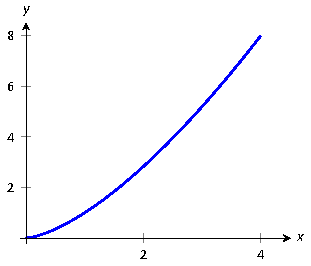
\includegraphics{figures/figarc1}
%\caption{A graph of $f(x) = x^{3/2}$ from Example~\ref{eg:6.3.1}.} \label{F:6.3.Ex1}
%\end{marginfigure}

 %EXAMPLE

\begin{activity} \label{A:6.4.1}  Consider the following situations in which mass is distributed in a non-constant manner.
\ba
	\item Suppose that a thin rod with constant cross-sectional area of 1 cm$^2$ has its mass distributed according to the density function $\rho(x) = 2e^{-0.2x}$, where $x$ is the distance in cm from the left end of the rod, and the units on $\rho(x)$ are g/cm.  If the rod is 10 cm long, determine the exact mass of the rod.
	
	\item Consider the cone that has a base of radius 4 m and a height of 5 m.  Picture the cone lying horizontally with the center of its base at the origin and think of the cone as a solid of revolution.  
	\begin{itemize}
		\item[i.]  Write and evaluate a definite integral whose value is the volume of the cone.

		\item[ii.]  Next, suppose that the cone has uniform density of 800 kg/m$^3$.  What is the mass of the solid cone?

		\item[iii.] Now suppose that the cone's density is not uniform, but rather that the cone is most dense at its base.  In particular, assume that the density of the cone is uniform across cross sections parallel to its base, but that in each such cross section that is a distance $x$ units from the origin, the density of the cross section is given by the function $\rho(x) = 400 + \frac{200}{1+x^2}$, measured in kg/m$^3$.  Determine and evaluate a definite integral whose value is the mass of this cone of non-uniform density.  Do so by first thinking about the mass of a given slice of the cone $x$ units away from the base; remember that in such a slice, the density will be \emph{essentially constant}.
	\end{itemize}

	\item Let a thin rod of constant cross-sectional area 1 cm$^2$ and length 12 cm have its mass be distributed according to the density function $\rho(x) = \frac{1}{25}(x-15)^2$, measured in g/cm.  Find the exact location $z$ at which to cut the bar so that the two pieces will each have identical mass.

\ea

\end{activity}
\begin{smallhint}
\ba
	\item Small hints for each of the prompts above.
\ea
\end{smallhint}
\begin{bighint}
\ba
	\item Big hints for each of the prompts above.
\ea
\end{bighint}
\begin{activitySolution}
\ba
	\item Solutions for each of the prompts above.
\ea
\end{activitySolution}
\aftera % ACTIVITY

%-------------------------------------------
% SUBSECTION WEIGHTED AVERAGES
%-------------------------------------------
\subsection*{Weighted Averages}

\begin{margintable}
\begin{center}
\begin{tabular}{ | l || c | c | c |}
   \hline 
   class & grade & grade points & credits  \\
   \hline \hline
   chemistry & B+ & $3.3$ & $5$ \\
   \hline
   calculus & A- & $3.7$ & $4$ \\
   \hline
   history & B- & $2.7$ & $3$ \\
   \hline
   psychology & B- & $2.7$ & $3$ \\
   \hline
\end{tabular} 
\end{center}
\caption{A college student's semester grades.} \label{T:6.3.grades}
\end{margintable}

The concept of an average is a natural one, and one that we have used repeatedly as part of our understanding of the meaning of the definite integral.  If we have $n$ values $a_1$, $a_2$, $\ldots$, $a_n$, we know that their average is given by
$$\frac{a_1 + a_2 + \cdots + a_n}{n},$$
and for a quantity being measured by a function $f$ on an interval $[a,b]$, the average value of the quantity on $[a,b]$ is
$$\frac{1}{b-a} \int_a^b f(x) \, dx.$$
As we continue to think about problems involving the distribution of mass, it is natural to consider the idea of a \emph{weighted} average, \index{weighted average} where certain quantities involved are counted more in the average.

A common use of weighted averages is in the computation of a student's GPA, where grades are weighted according to credit hours.  Let's consider the scenario in Table~\ref{T:6.3.grades}.

If all of the classes were of the same weight (i.e., the same number of credits), the student's GPA would simply be calculated by taking the average
$$\frac{3.3 + 3.7 + 2.7 + 2.7}{4} = 3.1.$$
But since the chemistry and calculus courses have higher weights (of $5$ and $4$ credits respectively), we actually compute the GPA according to the weighted average 
$$\frac{3.3 \cdot 5 + 3.7 \cdot 4 + 2.7 \cdot 3 + 2.7 \cdot 3}{5 + 4 + 3 + 3} = 3.1\overline{6}.$$
The weighted average reflects the fact that chemistry and calculus, as courses with higher credits, have a greater impact on the students' grade point average.  Note particularly that in the weighted average, each grade gets multiplied by its weight, and we divide by the sum of the weights.

In the following activity, we explore further how weighted averages can be used to find the balancing point of a physical system.

\begin{activity} \label{A:6.4.2} For quantities of equal weight, such as two children on a teeter-totter, the balancing point is found by taking the average of their locations.  When the weights of the quantities differ, we use a weighted average of their respective locations to find the balancing point. 
\ba
	\item Suppose that a shelf is 6 feet long, with its left end situated at $x = 0$.  If one book of weight 1 lb is placed at $x_1 = 0$, and another book of weight 1 lb is placed at $x_2 = 6$, what is the location of $\overline{x}$, the point at which the shelf would (theoretically) balance on a fulcrum?
	\item Now, say that we place four books on the shelf, each weighing 1 lb:  at $x_1 = 0$, at $x_2 = 2$, at $x_3 = 4$, and at $x_4 = 6$.  Find $\overline{x}$, the balancing point of the shelf.
	\item How does $\overline{x}$ change if we change the location of the third book?  Say the locations of the 1-lb books are  $x_1 = 0$, $x_2 = 2$, $x_3 = 3$, and $x_4 = 6$.  
	\item Next, suppose that we place four books on the shelf, but of varying weights:  at $x_1 = 0$ a 2-lb book, at $x_2 = 2$ a 3-lb book, and $x_3 = 4$ a 1-lb book, and at $x_4 = 6$ a 1-lb book.  Use a weighted average of the locations to find $\overline{x}$, the balancing point of the shelf.  How does the balancing point in this scenario compare to that found in (b)?
	\item What happens if we change the location of one of the books?  Say that we keep everything the same in (d), except that $x_3 = 5$.  How does $\overline{x}$ change?  
	\item What happens if we change the weight of one of the books?  Say that we keep everything the same in (d), except that the book at $x_3 = 4$ now weighs 2 lbs.  How does $\overline{x}$ change?
	\item Experiment with a couple of different scenarios of your choosing where you move the location of one of the books to the left, or you decrease the weight of one of the books.
	\item Write a couple of sentences to explain how adjusting the location of one of the books or the weight of one of the books affects the location of the balancing point of the shelf.  Think carefully here about how your changes should be considered relative to the location of the balancing point $\overline{x}$ of the current scenario.
\ea

\end{activity}
\begin{smallhint}
\ba
	\item Small hints for each of the prompts above.
\ea
\end{smallhint}
\begin{bighint}
\ba
	\item Big hints for each of the prompts above.
\ea
\end{bighint}
\begin{activitySolution}
\ba
	\item Solutions for each of the prompts above.
\ea
\end{activitySolution}
\aftera % ACTIVITY

%--------------------------------------
% SUBSECTION CENTER OF MASS
%--------------------------------------
\subsection*{Center of Mass} 

In Activity~\ref{A:6.4.2}, we saw that the balancing point of a system of point-masses\footnote{In the activity, we actually used \emph{weight} rather than \emph{mass}.  Since weight is computed by the gravitational constant times mass, the computations for the balancing point result in the same location regardless of whether we use weight or mass, since the gravitational constant is present in both the numerator and denominator of the weighted average.} (such as books on a shelf) is found by taking a weighted average of their respective locations.  In the activity, we were computing the \emph{center of mass} of a system of masses distributed along an axis, which is the balancing point of the axis on which the masses rest.

\definition{Center of Mass}{ % DEFINITION
For a collection of $n$ masses $m_1$, $\ldots$, $m_n$ that are distributed along a single axis at the locations $x_1$, $\ldots$, $x_n$, the \emph{center of mass} is given by
$$\overline{x} = \frac{x_1 m_1  + x_2 m_2 + \cdots x_n m_n}{m_1 + m_2 + \cdots + m_n}.$$
} % end definition

What if we instead consider a thin bar over which density is distributed continuously?  If the density is constant, it is obvious that the balancing point of the bar is its midpoint.  But if density is not constant, we must compute a weighted average.  Let's say that the function $\rho(x)$ tells us the density distribution along the bar, measured in g/cm.  If we slice the bar into small sections, this enables us to think of the bar as holding a collection of adjacent point-masses.  For a slice of thickness $\triangle x$ at location $x_i$, note that the mass of the slice, $m_i$, satisfies $m_i \approx \rho(x_i) \triangle x$.

\begin{marginfigure} % MARGIN FIGURE
\margingraphics{figures/6_3_Bar.eps}
\caption{A thin bar of constant cross-sectional area with density function $\rho(x)$ g/cm.} \label{F:6.3.Bar2}
\end{marginfigure}

Taking $n$ slices of the bar, we can approximate its center of mass by 
$$\overline{x} \approx \frac{x_1 \cdot \rho(x_1) \triangle x + x_2 \cdot \rho(x_2) \triangle x  + \cdots + x_n \cdot \rho(x_n) \triangle x }{\rho(x_1) \triangle x + \rho(x_2) \triangle x + \cdots + \rho(x_n) \triangle x}.$$
Rewriting the sums in sigma notation, it follows that
\begin{equation} \label{E:CtrOfM}
\overline{x} \approx \frac{\sum_{i = 1}^{n} x_i \cdot \rho(x_i) \triangle x}{\sum_{i = 1}^{n} \rho(x_i) \triangle x}.
\end{equation}
Moreover, it is apparent that the greater the number of slices, the more accurate our estimate of the balancing point will be, and that the sums in Equation~(\ref{E:CtrOfM}) can be viewed as Riemann sums.  Hence, in the limit as $n \to \infty$, we find that the center of mass is given by the quotient of two integrals.

\concept{Center of Mass}{ % CONCEPT
For a thin rod of density $\rho(x)$ distributed along an axis from $x = a$ to $x = b$, the center of mass of the rod is given by
$$\overline{x} = \frac{\int_a^b x \rho(x) \, dx}{\int_a^b \rho(x) \, dx}.$$
} % end concept

Note particularly that the denominator of $\overline{x}$ is the mass of the bar, and that this quotient of integrals is simply the continuous version of the weighted average of locations, $x$, along the bar.

\begin{example} \label{eg:6.4.2} % EXAMPLE
A thin bar occupies the interval $0 \leq x \leq 2$ and it has a density in kg/m of $\rho(x) = 1+ x^2$. Find the center of mass of the bar. 

\solution
From Example \ref{eg:6.4.1}, the mass of the bar in kilograms is $\frac{14}{3}$ kg. We just need to find $\int_a^b x \rho(x) \ dx$.
\begin{align*}
	\int_a^b \rho(x) \ dx  & = 	\int_0^2 x (1+x^2) \ dx \\
		&= \int_0^2 (x +x^3) \ dx \\
		&= 	\left(\frac{x^2}{2}+\frac{x^4}{4} \right) \Big|_0^2 \\
		&= 8.
\end{align*}
The center of mass, $\overline{x}$, 00is $\frac{8}{14/3} = \frac{12}{7}$. 

\end{example}

%\begin{marginfigure}[-8cm] %MARGIN FIGURE
%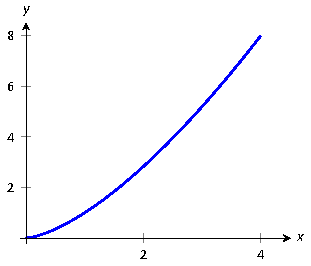
\includegraphics{figures/figarc1}
%\caption{A graph of $f(x) = x^{3/2}$ from Example~\ref{eg:6.3.1}.} \label{F:6.3.Ex1}
%\end{marginfigure}

 %EXAMPLE

\begin{activity} \label{A:6.4.3} Consider a thin bar of length 20 cm whose density is distributed according to the function $\rho(x) = 4 + 0.1x$, where $x = 0$ represents the left end of the bar.  Assume that $\rho$ is measured in g/cm and $x$ is measured in cm.
\ba
	\item Find the total mass, $M$, of the bar.
	\item Without doing any calculations, do you expect the center of mass of the bar to be equal to 10, less than 10, or greater than 10?  Why?
	\item Compute $\overline{x}$, the exact center of mass of the bar.
	\item What is the average density of the bar?  
	\item Now consider a different density function, given by $p(x) = 4e^{0.020732x}$, also for a bar of length 20 cm whose left end is at $x = 0$.  Plot both $\rho(x)$ and $p(x)$ on the same axes.  Without doing any calculations, which bar do you expect to have the greater center of mass?  Why?
	\item Compute the exact center of mass of the bar described in (e) whose density function is $p(x) = 4e^{0.020732x}$.  Check the result against the prediction you made in (e).
\ea

\end{activity}
\begin{smallhint}
\ba
	\item Small hints for each of the prompts above.
\ea
\end{smallhint}
\begin{bighint}
\ba
	\item Big hints for each of the prompts above.
\ea
\end{bighint}
\begin{activitySolution}
\ba
	\item Solutions for each of the prompts above.
\ea
\end{activitySolution}
\aftera % ACTIVITY

%-------------
% SUMMARY
%-------------
\begin{summary}
  \item For an object of constant density $D$, with volume $V$ and mass $m$, we know that $m = D \cdot V.$
  \item If an object with constant cross-sectional area (such as a thin bar) has its density distributed along an axis according to the function $\rho(x)$, then we can find the mass of the object between $x = a$ and $x = b$ by
  $$m = \int_a^b \rho(x) \, dx.$$
  \item For a system of point-masses distributed along an axis, say $m_1, \ldots, m_n$ at locations $x_1, \ldots, x_n$, the center of mass, $\overline{x}$, is given by the weighted average
  $$\overline{x} = \frac{\sum_{i=1}^n x_i m_i}{\sum_{i=1}^n m_i}.$$
  If instead we have mass continuously distributed along an axis, such as by a density function $\rho(x)$ for a thin bar of constant cross-sectional area, the center of mass of the portion of the bar between $x = a$ and $x = b$ is given by
  $$\overline{x} = \frac{\int_a^b x \rho(x) \, dx}{\int_a^b \rho(x) \, dx}.$$
  In each situation, $\overline{x}$ represents the balancing point of the system of masses or of the portion of the bar.
\end{summary}

\clearpage

%--------------
% EXERCISES
%--------------
\begin{adjustwidth*}{}{-2.25in}
\textbf{{\large Exercises}}
\setlength{\columnsep}{25pt}
\begin{multicols*}{2}
\noindent Terms and Concepts \small
\begin{enumerate}[1)]
\item T/F: The integral formula for computing Arc Length was found by first approximating arc length with straight line segments.
\item T/F: The integral formula for computing Arc Length includes a square--root, meaning the integration is probably easy.
\end{enumerate} 

\noindent {\normalsize Problems} \small

\begin{enumerate}[1),resume]
  \item Let a thin rod of length $a$ have density distribution function $\rho(x) = 10e^{-0.1x}$, where $x$ is measured in cm and $\rho$ in grams per centimeter.
  \ba
  	\item If the mass of the rod is 30 g, what is the value of $a$?
	\item For the 30g rod, will the center of mass lie at its midpoint, to the left of the midpoint, or to the right of the midpoint?  Why?
	\item For the 30g rod, find the center of mass, and compare your prediction in (b).
	\item At what value of $x$ should the 30g rod be cut in order to form two pieces of equal mass? 
  \ea
  
  \item Consider two thin bars of constant cross-sectional area, each of length 10 cm, with respective mass density functions $\rho(x) = \frac{1}{1+x^2}$ and $p(x) = e^{-0.1x}$.
  \ba
  	\item Find the mass of each bar.
	\item Find the center of mass of each bar.
	\item Now consider a new 10 cm bar whose mass density function is $f(x) = \rho(x) + p(x)$.  
	\be
		\item[i.]  Explain how you can easily find the mass of this new bar with little to no additional work.
		\item[ii.]  Similarly, compute $\int_0^{10} xf(x) \, dx$ as simply as possible, in light of earlier computations.
		\item[iii.]  True or false:  the center of mass of this new bar is the average of the centers of mass of the two earlier bars.  Write at least one sentence to say why your conclusion makes sense.
	\ee
  \ea
  
  \item Consider the curve given by $y = f(x) = 2xe^{-1.25x} + (30-x) e^{-0.25(30-x)}$.
  \ba
  	\item Plot this curve in the window $x = 0 \ldots 30$, $y = 0 \ldots 3$ (with constrained scaling so the units on the $x$ and $y$ axis are equal), and use it to generate a solid of revolution about the $x$-axis.  Explain why this curve could generate a reasonable model of a baseball bat.
	\item Let $x$ and $y$ be measured in inches.  Find the total volume of the baseball bat generated by revolving the given curve about the $x$-axis.  Include units on your answer
	\item Suppose that the baseball bat has constant weight density, and that the weight density is 0.6 ounces per cubic inch.  Find the total weight of the bat whose volume you found in (b).
	\item Because the baseball bat does not have constant cross-sectional area, we see that the amount of weight concentrated at a location $x$ along the bat is determined by the volume of a slice at location $x$.  Explain why we can think about the function $\rho(x) = 0.6 \pi f(x)^2$ (where $f$ is the function given at the start of the problem) as being the weight density function for how the weight of the baseball bat is distributed from $x = 0$ to $x = 30$.
	\item Compute the center of mass of the baseball bat.  
  \ea
\end{enumerate}

%------------------------------------------
% END OF EXERCISES ON FIRST PAGE
%------------------------------------------
\end{multicols*}
\end{adjustwidth*}

%\clearpage
%
%\begin{adjustwidth*}{}{-2.25in}
%\setlength{\columnsep}{25pt}
%\begin{multicols*}{2}\small
%
%\begin{enumerate}[1),start=12]
%
%\end{enumerate}
%
%%---------------------------------------------
%% END OF EXERCISES ON SECOND PAGE
%%---------------------------------------------
%\end{multicols*}
%\end{adjustwidth*}

\afterexercises 

\cleardoublepage